% THIS DATA IS COMPLETELY AI FABRICATED - NOT TO BE USED FOR REFERENCIAL PURPOSES 


\documentclass{article}
\usepackage{tikz}
\usepackage{pgfplots}
\pgfplotsset{compat=1.18}

\begin{document}

\begin{figure}[ht]
\centering
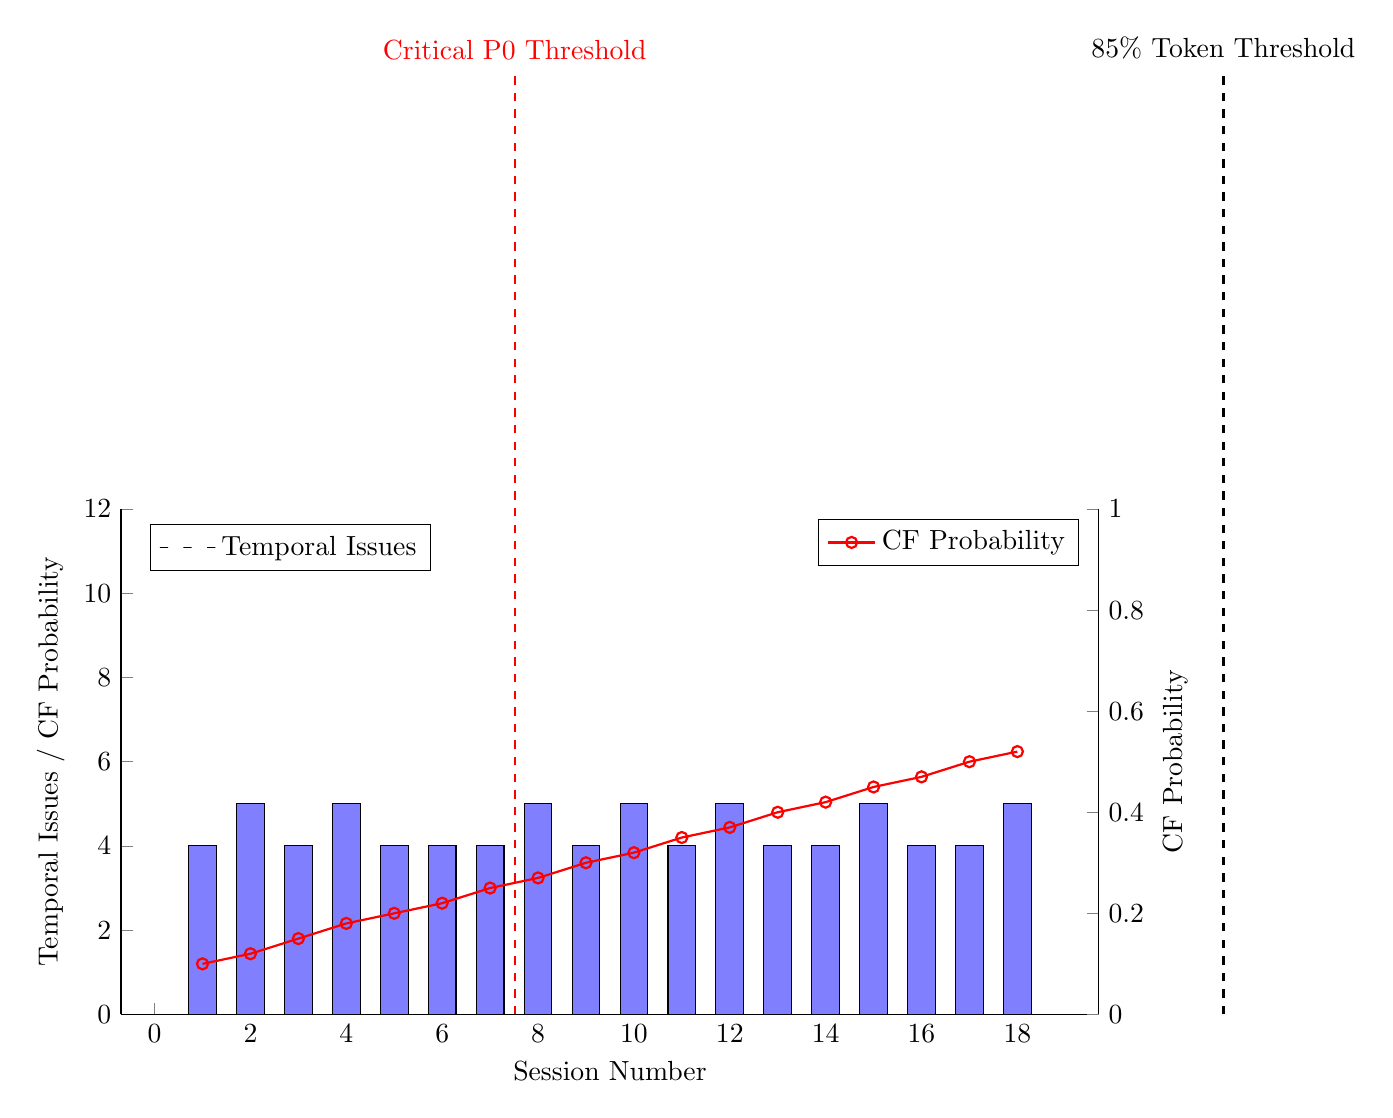
\begin{tikzpicture}

% Axes
\begin{axis}[
    width=14cm,
    height=8cm,
    xlabel={Session Number},
    ylabel={Temporal Issues / CF Probability},
    yticklabel style={/pgf/number format/fixed},
    ymax=12,
    ymin=0,
    axis y line*=left,
    axis x line*=bottom,
    legend pos=north west
]

% Temporal Issues per session (bars)
\addplot[ybar, fill=blue!50] coordinates {
    (1,4) (2,5) (3,4) (4,5) (5,4) (6,4) (7,4) (8,5)
    (9,4) (10,5) (11,4) (12,5) (13,4) (14,4) (15,5) (16,4) (17,4) (18,5)
};
\addlegendentry{Temporal Issues}

\end{axis}

% CF Probability line (secondary axis)
\begin{axis}[
    width=14cm,
    height=8cm,
    xlabel={Session Number},
    ylabel={CF Probability},
    axis y line*=right,
    axis x line=none,
    ymin=0,
    ymax=1,
]

\addplot[red, thick, mark=o] coordinates {
    (1,0.10) (2,0.12) (3,0.15) (4,0.18) (5,0.20) (6,0.22) (7,0.25) (8,0.27)
    (9,0.30) (10,0.32) (11,0.35) (12,0.37) (13,0.40) (14,0.42) (15,0.45) (16,0.47) (17,0.50) (18,0.52)
};
\addlegendentry{CF Probability}

\end{axis}

% Optional threshold lines
\draw[thick, dashed, red] (5,0) -- (5,12) node[above] {Critical P0 Threshold};
\draw[thick, dashed, black] (14,0) -- (14,12) node[above] {85\% Token Threshold};

\end{tikzpicture}
\caption{Mockup AI Monitoring Dashboard: Temporal Issues per Session (bars), Catastrophic Failure Probability (line), with key operational thresholds.}
\end{figure}

\end{document}
